\documentclass{report}
\usepackage[spanish]{babel}
\usepackage[left=2.5cm, right=2.5cm, top=3cm, bottom=3cm]{geometry}
\usepackage{enumerate}
\usepackage{graphicx}
\usepackage{booktabs}
\usepackage{tabularx}
\usepackage{enumitem}
\usepackage{amsmath}
\usepackage{amsfonts}
\usepackage{float}
\usepackage{hyperref} 
\usepackage[utf8]{inputenc}
\usepackage{multirow}
\usepackage{array}
\usepackage{geometry}
\usepackage{graphicx}
\geometry{a4paper, margin=1in}



\setlength{\parindent}{0pt}

\begin{document}

    \begin{titlepage}
        \centering
        {\bfseries\Huge Informe Técnico \par}
        \vspace*{1cm}
        \vspace*{3cm}
        \vspace*{1cm}
        {\LARGE \textbf{Nombre: Gestión de campeonatos de béisbol} }
        \vfill
        {\bfseries\LARGE Autores: \par}
        {\Large Ariadna Vel\'azquez Rey  C311 \par} 
        {\Large L\'ia L\'opez Rosales  C312 \par} 
        {\Large Carlos Daniel Largacha Leal  C312 \par} 
        {\Large Gabriel Andr\'es Pla Lasa  C311 \par} 
        {\Large Raidel Miguel Cabellud Lizaso C311 \par} 
        \vfill
    \end{titlepage}

    \section*{Diccionario de datos}    
    \subsection*{Tabla: User}
    \begin{tabular}{|>{\raggedright\arraybackslash}p{3cm}|>{\raggedright\arraybackslash}p{3cm}|>{\raggedright\arraybackslash}p{6cm}|>{\raggedright\arraybackslash}p{4cm}|}
        \hline
        \textbf{Campo} & \textbf{Tipo de Dato} & \textbf{Descripción} & \textbf{Restricciones} \\
        \hline
        id & AutoField (PK) & Identificador único del usuario. & Primary Key \\
        \hline
        email & EmailField & Correo electrónico del usuario. & Único, máximo 255 caracteres. \\
        \hline
        rol\_id & ForeignKey (Rol) & Rol asignado al usuario. & No nulo, relación con la tabla \texttt{Rol}. \\
        \hline
        TD\_id & ForeignKey (TechnicalDirector) & Director técnico asociado al usuario. & Nulo permitido, relación con \texttt{TechnicalDirector}. \\
        \hline
        password & CharField & Contraseña del usuario. & Máximo 128 caracteres. \\
        \hline
    \end{tabular}
    
    \textbf{Restricciones adicionales:}
    \begin{itemize}
        \item El campo \texttt{TD\_id} no puede ser nulo si el \texttt{rol\_id} es "Director Técnico".
    \end{itemize}
    
    ---
    
    \subsection*{Tabla: Rol}
    \begin{tabular}{|>{\raggedright\arraybackslash}p{3cm}|>{\raggedright\arraybackslash}p{3cm}|>{\raggedright\arraybackslash}p{6cm}|>{\raggedright\arraybackslash}p{4cm}|}
        \hline
        \textbf{Campo} & \textbf{Tipo de Dato} & \textbf{Descripción} & \textbf{Restricciones} \\
        \hline
        id & AutoField (PK) & Identificador único del rol. & Primary Key \\
        \hline
        type & CharField & Tipo de rol (Director Técnico, Admin, Usuario). & Máximo 50 caracteres, opciones predefinidas. \\
        \hline
    \end{tabular}
    
    ---
    
    \subsection*{Tabla: TechnicalDirector}
    \begin{tabular}{|>{\raggedright\arraybackslash}p{3cm}|>{\raggedright\arraybackslash}p{3cm}|>{\raggedright\arraybackslash}p{6cm}|>{\raggedright\arraybackslash}p{4cm}|}
        \hline
        \textbf{Campo} & \textbf{Tipo de Dato} & \textbf{Descripción} & \textbf{Restricciones} \\
        \hline
        id & AutoField (PK) & Identificador único del director técnico. & Primary Key \\
        \hline
        direction\_team & ForeignKey (DirectionTeam) & Equipo de dirección asociado. & Nulo permitido, relación con \texttt{DirectionTeam}. \\
        \hline
        W\_id & ForeignKey (Worker) & Trabajador asociado al director técnico. & No nulo, relación con \texttt{Worker}. \\
        \hline
    \end{tabular}
    
    \textbf{Restricciones adicionales:}
    \begin{itemize}
        \item Clave primaria compuesta: \texttt{W\_id} e \texttt{id}.
    \end{itemize}
    
    ---
    
    \subsection*{Tabla: Worker}
    \begin{tabular}{|>{\raggedright\arraybackslash}p{3cm}|>{\raggedright\arraybackslash}p{3cm}|>{\raggedright\arraybackslash}p{6cm}|>{\raggedright\arraybackslash}p{4cm}|}
        \hline
        \textbf{Campo} & \textbf{Tipo de Dato} & \textbf{Descripción} & \textbf{Restricciones} \\
        \hline
        id & AutoField (PK) & Identificador único del trabajador. & Primary Key \\
        \hline
        P\_id & ForeignKey (Person) & Persona asociada al trabajador. & No nulo, relación con \texttt{Person}. \\
        \hline
        DT\_id & ForeignKey (DirectionTeam) & Equipo de dirección asociado. & Nulo permitido, relación con \texttt{DirectionTeam}. \\
        \hline
    \end{tabular}
    
    \textbf{Restricciones adicionales:}
    \begin{itemize}
        \item Clave primaria compuesta: \texttt{P\_id} e \texttt{id}.
    \end{itemize}
    
    ---
    
    \subsection*{Tabla: DirectionTeam}
    \begin{tabular}{|>{\raggedright\arraybackslash}p{3cm}|>{\raggedright\arraybackslash}p{3cm}|>{\raggedright\arraybackslash}p{6cm}|>{\raggedright\arraybackslash}p{4cm}|}
        \hline
        \textbf{Campo} & \textbf{Tipo de Dato} & \textbf{Descripción} & \textbf{Restricciones} \\
        \hline
        id & AutoField (PK) & Identificador único del equipo de dirección. & Primary Key \\
        \hline
        Team\_id & ForeignKey (Team) & Equipo asociado al equipo de dirección. & No nulo, relación con \texttt{Team}. \\
        \hline
    \end{tabular}
    
    ---
    
    \subsection*{Tabla: Team}
    \begin{tabular}{|>{\raggedright\arraybackslash}p{3cm}|>{\raggedright\arraybackslash}p{3cm}|>{\raggedright\arraybackslash}p{6cm}|>{\raggedright\arraybackslash}p{4cm}|}
        \hline
        \textbf{Campo} & \textbf{Tipo de Dato} & \textbf{Descripción} & \textbf{Restricciones} \\
        \hline
        id & AutoField (PK) & Identificador único del equipo. & Primary Key \\
        \hline
        name & CharField & Nombre del equipo. & Máximo 100 caracteres. \\
        \hline
        color & CharField & Color del equipo. & Máximo 50 caracteres. \\
        \hline
        initials & CharField & Iniciales del equipo. & Máximo 10 caracteres. \\
        \hline
        representative\_entity & CharField & Entidad representativa del equipo. & Máximo 100 caracteres. \\
        \hline
    \end{tabular}
    
    ---
    
    \subsection*{Tabla: Person}
    \begin{tabular}{|>{\raggedright\arraybackslash}p{3cm}|>{\raggedright\arraybackslash}p{3cm}|>{\raggedright\arraybackslash}p{6cm}|>{\raggedright\arraybackslash}p{4cm}|}
        \hline
        \textbf{Campo} & \textbf{Tipo de Dato} & \textbf{Descripción} & \textbf{Restricciones} \\
        \hline
        id & AutoField (PK) & Identificador único de la persona. & Primary Key \\
        \hline
        CI & IntegerField & Cédula de identidad de la persona. & Único. \\
        \hline
        age & IntegerField & Edad de la persona. &  \\
        \hline
        name & CharField & Nombre de la persona. & Máximo 100 caracteres. \\
        \hline
        lastname & CharField & Apellido de la persona. & Máximo 100 caracteres. \\
        \hline
    \end{tabular}
    
    ---
    
    \subsection*{Tabla: Position}
    \begin{tabular}{|>{\raggedright\arraybackslash}p{3cm}|>{\raggedright\arraybackslash}p{3cm}|>{\raggedright\arraybackslash}p{6cm}|>{\raggedright\arraybackslash}p{4cm}|}
        \hline
        \textbf{Campo} & \textbf{Tipo de Dato} & \textbf{Descripción} & \textbf{Restricciones} \\
        \hline
        id & AutoField (PK) & Identificador único de la posición. & Primary Key \\
        \hline
        name & CharField & Nombre de la posición. & Máximo 100 caracteres. \\
        \hline
    \end{tabular}
    
    ---
    
    \subsection*{Tabla: BaseballPlayer}
    \begin{tabular}{|>{\raggedright\arraybackslash}p{3cm}|>{\raggedright\arraybackslash}p{3cm}|>{\raggedright\arraybackslash}p{6cm}|>{\raggedright\arraybackslash}p{4cm}|}
        \hline
        \textbf{Campo} & \textbf{Tipo de Dato} & \textbf{Descripción} & \textbf{Restricciones} \\
        \hline
        id & AutoField (PK) & Identificador único del pelotero. & Primary Key \\
        \hline
        P\_id & ForeignKey (Person) & Persona asociada al pelotero. & No nulo, relación con \texttt{Person}. \\
        \hline
        batting\_average & FloatField & Promedio de bateo del pelotero. &  \\
        \hline
        years\_of\_experience & IntegerField & Años de experiencia del pelotero. &  \\
        \hline
        pitcher & ForeignKey (Pitcher) & Lanzador asociado al pelotero. & Nulo permitido, relación con \texttt{Pitcher}. \\
        \hline
    \end{tabular}
    
    ---
    
    \subsection*{Tabla: Pitcher}
    \begin{tabular}{|>{\raggedright\arraybackslash}p{3cm}|>{\raggedright\arraybackslash}p{3cm}|>{\raggedright\arraybackslash}p{6cm}|>{\raggedright\arraybackslash}p{4cm}|}
        \hline
        \textbf{Campo} & \textbf{Tipo de Dato} & \textbf{Descripción} & \textbf{Restricciones} \\
        \hline
        P\_id & ForeignKey (BaseballPlayer) & Pelotero asociado al lanzador. & No nulo, relación con \texttt{BaseballPlayer}. \\
        \hline
        dominant\_hand & CharField & Mano dominante del lanzador. & Opciones: 'izquierda', 'derecha', 'ambas'. \\
        \hline
        No\_games\_won & PositiveIntegerField & Número de juegos ganados. &  \\
        \hline
        No\_games\_lost & PositiveIntegerField & Número de juegos perdidos. &  \\
        \hline
        running\_average & PositiveIntegerField & Promedio de carreras permitidas. &  \\
        \hline
    \end{tabular}
    
    ---
    
    \subsection*{Tabla: BPParticipation}
    \begin{tabular}{|>{\raggedright\arraybackslash}p{3cm}|>{\raggedright\arraybackslash}p{3cm}|>{\raggedright\arraybackslash}p{6cm}|>{\raggedright\arraybackslash}p{4cm}|}
        \hline
        \textbf{Campo} & \textbf{Tipo de Dato} & \textbf{Descripción} & \textbf{Restricciones} \\
        \hline
        BP\_id & ForeignKey (BaseballPlayer) & Pelotero que participa en la serie. & No nulo, relación con \texttt{BaseballPlayer}. \\
        \hline
        series & ForeignKey (Series) & Serie en la que participa el pelotero. & No nulo, relación con \texttt{Series}. \\
        \hline
        team\_id & ForeignKey (Team) & Equipo al que pertenece el pelotero. & No nulo, relación con \texttt{Team}. \\
        \hline
    \end{tabular}
    
    \textbf{Restricciones adicionales:}
    \begin{itemize}
        \item Clave primaria compuesta: \texttt{BP\_id} y \texttt{series}.
    \end{itemize}
    
    ---
    
    \subsection*{Tabla: LineUp}
    \begin{tabular}{|>{\raggedright\arraybackslash}p{3cm}|>{\raggedright\arraybackslash}p{3cm}|>{\raggedright\arraybackslash}p{6cm}|>{\raggedright\arraybackslash}p{4cm}|}
        \hline
        \textbf{Campo} & \textbf{Tipo de Dato} & \textbf{Descripción} & \textbf{Restricciones} \\
        \hline
        id & AutoField (PK) & Identificador único de la alineación. & Primary Key \\
        \hline
        team\_id & ForeignKey (Team) & Equipo asociado a la alineación. & No nulo, relación con \texttt{Team}. \\
        \hline
    \end{tabular}
    
    \textbf{Restricciones adicionales:}
    \begin{itemize}
        \item Clave primaria compuesta: \texttt{id} y \texttt{team\_id}.
    \end{itemize}
    
    ---
    
    \subsection*{Tabla: PlayerInLineUp}
    \begin{tabular}{|>{\raggedright\arraybackslash}p{3cm}|>{\raggedright\arraybackslash}p{3cm}|>{\raggedright\arraybackslash}p{6cm}|>{\raggedright\arraybackslash}p{4cm}|}
        \hline
        \textbf{Campo} & \textbf{Tipo de Dato} & \textbf{Descripción} & \textbf{Restricciones} \\
        \hline
        line\_up & ForeignKey (LineUp) & Alineación a la que pertenece el jugador. & No nulo, relación con \texttt{LineUp}. \\
        \hline
        player\_in\_position & ForeignKey (PlayerInPosition) & Jugador en una posición específica. & No nulo, relación con \texttt{PlayerInPosition}. \\
        \hline
    \end{tabular}
    
    \textbf{Restricciones adicionales:}
    \begin{itemize}
        \item Clave primaria compuesta: \texttt{line\_up} y \texttt{player\_in\_position}.
    \end{itemize}
    
    ---
    
    \subsection*{Tabla: PlayerInPosition}
    \begin{tabular}{|>{\raggedright\arraybackslash}p{3cm}|>{\raggedright\arraybackslash}p{3cm}|>{\raggedright\arraybackslash}p{6cm}|>{\raggedright\arraybackslash}p{4cm}|}
        \hline
        \textbf{Campo} & \textbf{Tipo de Dato} & \textbf{Descripción} & \textbf{Restricciones} \\
        \hline
        BP\_id & ForeignKey (BaseballPlayer) & Pelotero en una posición. & No nulo, relación con \texttt{BaseballPlayer}. \\
        \hline
        position & ForeignKey (Position) & Posición del pelotero. & No nulo, relación con \texttt{Position}. \\
        \hline
        effectiveness & FloatField & Efectividad del pelotero en la posición. &  \\
        \hline
    \end{tabular}
    
    \textbf{Restricciones adicionales:}
    \begin{itemize}
        \item Clave primaria compuesta: \texttt{BP\_id} y \texttt{position}.
    \end{itemize}
    
    ---
    
    \subsection*{Tabla: Season}
    \begin{tabular}{|>{\raggedright\arraybackslash}p{3cm}|>{\raggedright\arraybackslash}p{3cm}|>{\raggedright\arraybackslash}p{6cm}|>{\raggedright\arraybackslash}p{4cm}|}
        \hline
        \textbf{Campo} & \textbf{Tipo de Dato} & \textbf{Descripción} & \textbf{Restricciones} \\
        \hline
        id & AutoField (PK) & Identificador único de la temporada. & Primary Key \\
        \hline
        name & CharField & Nombre de la temporada. &  \\
        \hline
    \end{tabular}
    
    ---
    
    \subsection*{Tabla: Series}
    \begin{tabular}{|>{\raggedright\arraybackslash}p{3cm}|>{\raggedright\arraybackslash}p{3cm}|>{\raggedright\arraybackslash}p{6cm}|>{\raggedright\arraybackslash}p{4cm}|}
        \hline
        \textbf{Campo} & \textbf{Tipo de Dato} & \textbf{Descripción} & \textbf{Restricciones} \\
        \hline
        id & AutoField (PK) & Identificador único de la serie. & Primary Key \\
        \hline
        season & ForeignKey (Season) & Temporada a la que pertenece la serie. & No nulo, relación con \texttt{Season}. \\
        \hline
        name & CharField & Nombre de la serie. & Máximo 100 caracteres. \\
        \hline
        type & CharField & Tipo de serie. & Máximo 50 caracteres. \\
        \hline
        init\_date & DateTimeField & Fecha de inicio de la serie. &  \\
        \hline
        end\_date & DateTimeField & Fecha de finalización de la serie. &  \\
        \hline
    \end{tabular}
    
    \textbf{Restricciones adicionales:}
    \begin{itemize}
        \item Clave primaria compuesta: \texttt{season} e \texttt{id}.
        \item \texttt{init\_date} debe ser anterior a \texttt{end\_date}.
    \end{itemize}
    
    ---
    
    \subsection*{Tabla: Game}
    \begin{tabular}{|>{\raggedright\arraybackslash}p{3cm}|>{\raggedright\arraybackslash}p{3cm}|>{\raggedright\arraybackslash}p{6cm}|>{\raggedright\arraybackslash}p{4cm}|}
        \hline
        \textbf{Campo} & \textbf{Tipo de Dato} & \textbf{Descripción} & \textbf{Restricciones} \\
        \hline
        id & AutoField (PK) & Identificador único del juego. & Primary Key \\
        \hline
        local & ForeignKey (TeamOnTheField) & Equipo local. & No nulo, relación con \texttt{TeamOnTheField}. \\
        \hline
        date & DateTimeField & Fecha del juego. &  \\
        \hline
        rival & ForeignKey (TeamOnTheField) & Equipo rival. & No nulo, relación con \texttt{TeamOnTheField}. \\
        \hline
        series & ForeignKey (Series) & Serie a la que pertenece el juego. & No nulo, relación con \texttt{Series}. \\
        \hline
        score & ForeignKey (Score) & Puntuación del juego. & Nulo permitido, relación con \texttt{Score}. \\
        \hline
    \end{tabular}
    
    \textbf{Restricciones adicionales:}
    \begin{itemize}
        \item Clave primaria compuesta: \texttt{local} y \texttt{date}.
        \item \texttt{local} no puede ser igual a \texttt{rival}.
    \end{itemize}
    
    ---
    
    \subsection*{Tabla: Score}
    \begin{tabular}{|>{\raggedright\arraybackslash}p{3cm}|>{\raggedright\arraybackslash}p{3cm}|>{\raggedright\arraybackslash}p{6cm}|>{\raggedright\arraybackslash}p{4cm}|}
        \hline
        \textbf{Campo} & \textbf{Tipo de Dato} & \textbf{Descripción} & \textbf{Restricciones} \\
        \hline
        id & AutoField (PK) & Identificador único del marcador. & Primary Key \\
        \hline
        winner & ForeignKey (Team) & Equipo ganador. & No nulo, relación con \texttt{Team}. \\
        \hline
        loser & ForeignKey (Team) & Equipo perdedor. & No nulo, relación con \texttt{Team}. \\
        \hline
        w\_points & PositiveIntegerField & Puntos del equipo ganador. &  \\
        \hline
        l\_points & PositiveIntegerField & Puntos del equipo perdedor. &  \\
        \hline
    \end{tabular}
    
    \textbf{Restricciones adicionales:}
    \begin{itemize}
        \item \texttt{winner} no puede ser igual a \texttt{loser}.
        \item \texttt{w\_points} debe ser mayor o igual a \texttt{l\_points}.
    \end{itemize}
    
    ---
    
    \subsection*{Tabla: PlayerSwap}
    \begin{tabular}{|>{\raggedright\arraybackslash}p{3cm}|>{\raggedright\arraybackslash}p{3cm}|>{\raggedright\arraybackslash}p{6cm}|>{\raggedright\arraybackslash}p{4cm}|}
        \hline
        \textbf{Campo} & \textbf{Tipo de Dato} & \textbf{Descripción} & \textbf{Restricciones} \\
        \hline
        id & AutoField (PK) & Identificador único del cambio. & Primary Key \\
        \hline
        old\_player & ForeignKey (BaseballPlayer) & Jugador reemplazado. & No nulo, relación con \texttt{BaseballPlayer}. \\
        \hline
        date & DateTimeField & Fecha del cambio. &  \\
        \hline
        new\_player & ForeignKey (BaseballPlayer) & Jugador que entra. & No nulo, relación con \texttt{BaseballPlayer}. \\
        \hline
        position & ForeignKey (Position) & Posición del cambio. & No nulo, relación con \texttt{Position}. \\
        \hline
        game\_team & ForeignKey (TeamOnTheField) & Equipo en el campo. & No nulo, relación con \texttt{TeamOnTheField}. \\
        \hline
    \end{tabular}
    
    \textbf{Restricciones adicionales:}
    \begin{itemize}
        \item Clave primaria compuesta: \texttt{old\_player} y \texttt{date}.
    \end{itemize}
    
    ---
    
    \subsection*{Tabla: StarPlayer}
    \begin{tabular}{|>{\raggedright\arraybackslash}p{3cm}|>{\raggedright\arraybackslash}p{3cm}|>{\raggedright\arraybackslash}p{6cm}|>{\raggedright\arraybackslash}p{4cm}|}
        \hline
        \textbf{Campo} & \textbf{Tipo de Dato} & \textbf{Descripción} & \textbf{Restricciones} \\
        \hline
        id & AutoField (PK) & Identificador único del jugador estrella. & Primary Key \\
        \hline
        series & ForeignKey (Series) & Serie en la que es jugador estrella. & No nulo, relación con \texttt{Series}. \\
        \hline
        position & ForeignKey (Position) & Posición del jugador estrella. & No nulo, relación con \texttt{Position}. \\
        \hline
        BP\_id & ForeignKey (BaseballPlayer) & Pelotero estrella. & No nulo, relación con \texttt{BaseballPlayer}. \\
        \hline
    \end{tabular}
    
    \textbf{Restricciones adicionales:}
    \begin{itemize}
        \item Clave primaria compuesta: \texttt{series} y \texttt{position}.
    \end{itemize}
    
    ---
    
    \subsection*{Tabla: TeamOnTheField}
    \begin{tabular}{|>{\raggedright\arraybackslash}p{3cm}|>{\raggedright\arraybackslash}p{3cm}|>{\raggedright\arraybackslash}p{6cm}|>{\raggedright\arraybackslash}p{4cm}|}
        \hline
        \textbf{Campo} & \textbf{Tipo de Dato} & \textbf{Descripción} & \textbf{Restricciones} \\
        \hline
        id & AutoField (PK) & Identificador único del equipo en el campo. & Primary Key \\
        \hline
        lineup\_id & ForeignKey (LineUp) & Alineación asociada al equipo en el campo. & No nulo, relación con \texttt{LineUp}. \\
        \hline
    \end{tabular}
    
    ---
    
    \section*{Esquema con el diseño de la aplicación}
    \begin{figure}[h]
        \centering
        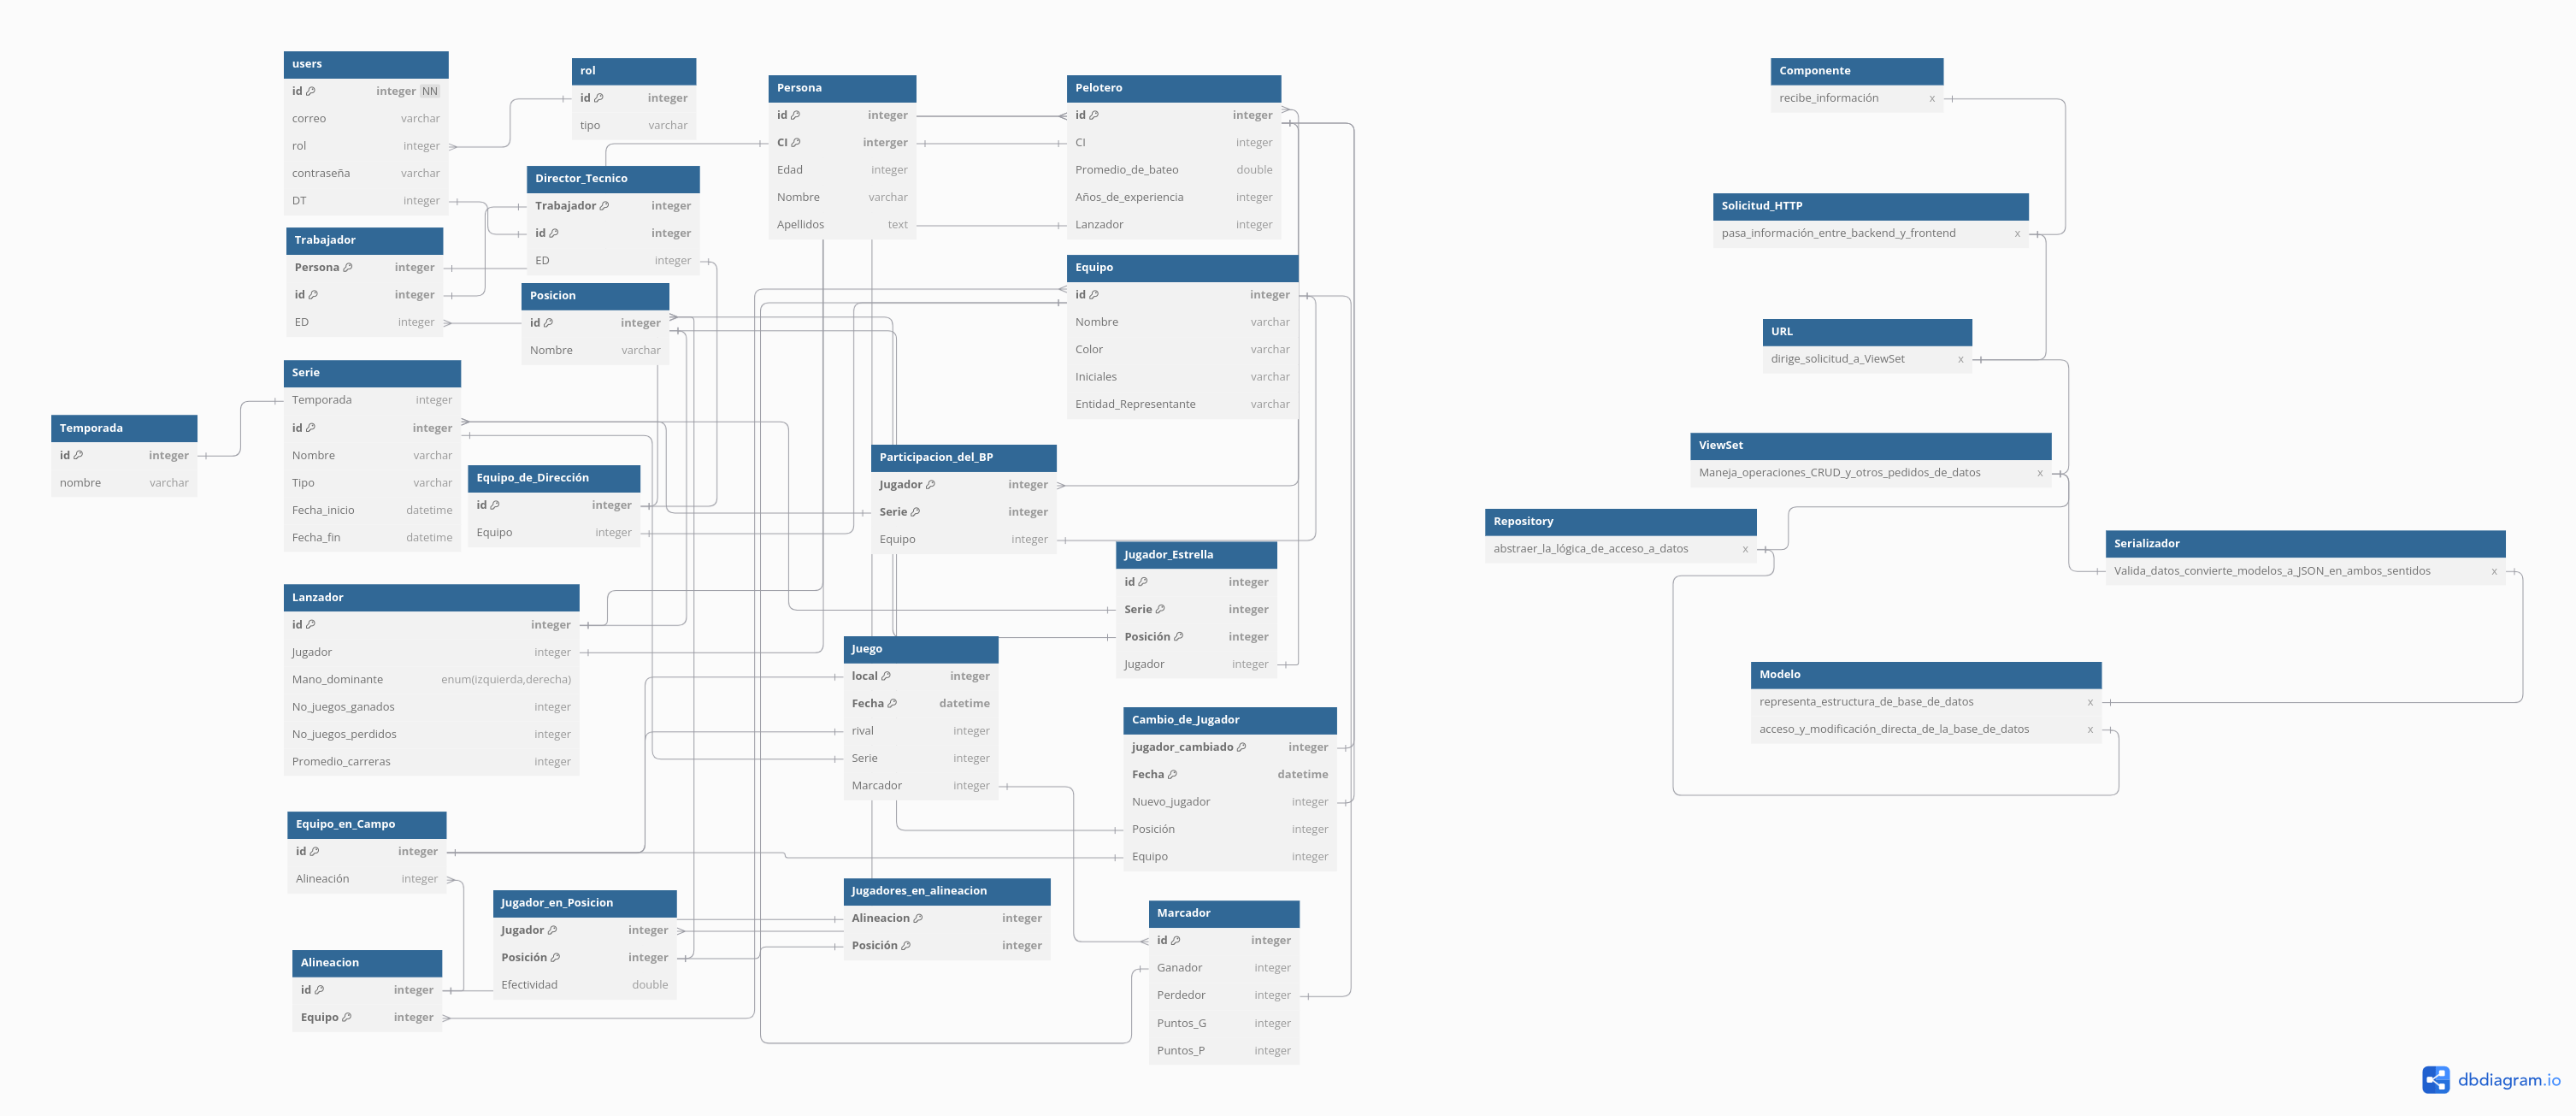
\includegraphics[width=0.8\textwidth]{Copy of Gestion_de_campeonatos_de_beisbol.png}
        \caption{Diagrama de gestión de campeonatos de béisbol}
        \label{fig:gestion_campeonatos}
    \end{figure}
    La aplicación sigue un flujo cliente-servidor, donde el frontend (React) y el backend (Django Rest Framework) se comunican a través de solicitudes HTTP. A continuación, se describe el flujo de información y procesamiento en cada capa de la aplicación:

    \section*{Frontend (React)}
    El frontend es responsable de la interfaz de usuario (UI) y la interacción con el usuario. Está construido con React, una biblioteca de JavaScript que permite crear interfaces dinámicas y reactivas. El flujo en el frontend es el siguiente:
    
    \subsection*{Interfaz de Usuario (UI)}
    \begin{itemize}
        \item React renderiza componentes que representan la interfaz gráfica de la aplicación.
        \item Los componentes pueden ser formularios, listas, tablas, botones, etc., que permiten al usuario interactuar con la aplicación.
    \end{itemize}
    
    \subsection*{Gestión del Estado}
    \begin{itemize}
        \item React utiliza un sistema de estado (por ejemplo, con \texttt{useState}, \texttt{useReducer} o bibliotecas como Redux) para manejar los datos que se muestran en la interfaz.
        \item El estado se actualiza dinámicamente en respuesta a las acciones del usuario (por ejemplo, hacer clic en un botón o enviar un formulario).
    \end{itemize}
    
    \subsection*{Comunicación con el Backend}
    \begin{itemize}
        \item Cuando el usuario realiza una acción que requiere datos del servidor (por ejemplo, cargar una lista de equipos o enviar un formulario), React realiza una solicitud HTTP (GET, POST, PUT, DELETE) al backend a través de la API REST.
        \item Para realizar estas solicitudes, se utiliza \texttt{fetch} o bibliotecas como Axios.
    \end{itemize}
    
    \subsection*{Renderizado Dinámico}
    \begin{itemize}
        \item Una vez que el backend responde con los datos solicitados, React actualiza el estado de la aplicación y re-renderiza los componentes para reflejar los cambios en la interfaz.
    \end{itemize}
    
    \section*{Backend (Django Rest Framework)}
    El backend es responsable de la lógica de negocio, el procesamiento de datos y la comunicación con la base de datos. Está construido con Django Rest Framework (DRF), que proporciona herramientas para crear APIs RESTful de manera eficiente. El flujo en el backend es el siguiente:
    
    \subsection*{Solicitud HTTP}
    \begin{itemize}
        \item Cuando el frontend realiza una solicitud HTTP (por ejemplo, una petición GET para obtener datos o POST para enviar datos), Django recibe la solicitud y la procesa.
    \end{itemize}
    
    \subsection*{Enrutamiento (URLs)}
    \begin{itemize}
        \item Django utiliza un sistema de enrutamiento (definido en el archivo \texttt{urls.py}) para dirigir la solicitud al ViewSet o Vista correspondiente.
    \end{itemize}
    
    \subsection*{Vistas (Viewsets)}
    \begin{itemize}
        \item Los ViewSets (o Vistas) son responsables de manejar la lógica de la solicitud. En DRF, los ViewSets permiten realizar operaciones CRUD (Crear, Leer, Actualizar, Eliminar) de manera simplificada.
        \item Las vistas interactúan con los serializadores para validar y transformar los datos entrantes o salientes.
    \end{itemize}
    
    \subsection*{Serializadores}
    Los serializadores en DRF son responsables de:
    \begin{itemize}
        \item Validar los datos enviados por el frontend (por ejemplo, datos de un formulario).
        \item Convertir los objetos de Django (modelos) en formatos como JSON para enviarlos al frontend.
        \item Convertir los datos JSON recibidos del frontend en objetos de Django para su procesamiento.
    \end{itemize}
    
    \subsection*{Modelos y Base de Datos}
    \begin{itemize}
        \item Los modelos de Django representan la estructura de la base de datos. Cada modelo define una tabla y sus campos.
        \item Cuando es necesario acceder o modificar datos, las vistas interactúan con los modelos a través del ORM (Object-Relational Mapping) de Django.
        \item El ORM permite realizar consultas a la base de datos sin escribir SQL directamente, lo que simplifica el manejo de datos.
    \end{itemize}
    
    \subsection*{Repositorios}
    \begin{itemize}
        \item Se utilizan repositorios para abstraer la lógica de acceso a datos. Los repositorios actúan como una capa intermedia entre las vistas y los modelos, centralizando las operaciones de la base de datos.
    \end{itemize}
    
    \subsection*{Respuesta HTTP}
    \begin{itemize}
        \item Una vez que la vista procesa la solicitud y obtiene los datos necesarios, devuelve una respuesta HTTP al frontend. Esta respuesta suele ser un objeto JSON que contiene los datos solicitados o un mensaje de confirmación.
    \end{itemize}
    
    \section*{Flujo Completo de una Solicitud}
    A continuación, se describe el flujo completo de una solicitud típica en la aplicación:
    
    \begin{enumerate}
        \item \textbf{Usuario realiza una acción en el frontend:}
        \begin{itemize}
            \item Por ejemplo, el usuario hace clic en un botón para cargar una lista de equipos.
        \end{itemize}
        \item \textbf{React realiza una solicitud HTTP:}
        \begin{itemize}
            \item React utiliza Axios o \texttt{fetch} para enviar una solicitud GET al endpoint correspondiente en el backend (por ejemplo, \texttt{/api/teams/}).
        \end{itemize}
        \item \textbf{Django recibe la solicitud:}
        \begin{itemize}
            \item Django dirige la solicitud al ViewSet correspondiente a través del archivo \texttt{urls.py}.
        \end{itemize}
        \item \textbf{ViewSet procesa la solicitud:}
        \begin{itemize}
            \item El ViewSet utiliza el serializador para obtener los datos de la base de datos a través del modelo.
            \item El serializador convierte los objetos de Django en JSON.
        \end{itemize}
        \item \textbf{Respuesta al frontend:}
        \begin{itemize}
            \item El ViewSet devuelve una respuesta HTTP con los datos en formato JSON.
        \end{itemize}
        \item \textbf{React actualiza el estado y la interfaz:}
        \begin{itemize}
            \item React recibe la respuesta, actualiza el estado de la aplicación y re-renderiza los componentes para mostrar los datos al usuario.
        \end{itemize}
    \end{enumerate}
    \section*{Esquema de las clases definidas}

    \section*{Solución propuesta}

    \section*{Otras informaciones relevantes}



\end{document}